\pdfsuppresswarningpagegroup=1

\documentclass{article}

\usepackage{amsmath}
\usepackage{multicol}
\usepackage{multirow}
\usepackage{makecell}
\usepackage{graphicx}
\usepackage[subrefformat=simple,labelformat=simple]{subcaption}
\usepackage{hyperref}
\usepackage{cleveref}
\usepackage{siunitx}
\usepackage{todonotes}
\usepackage[shortlabels]{enumitem}
\usepackage[margin=1in]{geometry}
\renewcommand\thesubfigure{(\alph{subfigure})}

\newcommand{\svec}[1]{{\vec{#1}\mkern2mu\vphantom{#1}}}
\newcommand{\pvec}[1]{\svec^\prime}
\newcommand{\matrixbold}[1]{\mathbf{#1}}

\newcommand{\M}[2]{\texttt{M#1\_#2}}

\begin{document}
	
\title{Alignment and stitching of microscope images}
\author{Heshy Roskes}
\date{March 18, 2020}

\section{Introduction}

Our microscope is supposed to scan a tissue sample, which covers some subset of a slide of size $L\times W$.  Initially, it performs a quick scan of the whole slide with a small magnification setting.  This scan is recorded in \texttt{qptiff} format.

Using that image, the microscope determines which parts of the slide actually have tissue in them.  It scans those sections under a larger magnification, using high-powered fields of size $l\times w$.  Covering the whole tissue may require $O(1000)$ fields.

The scanning is configured with an overlap fraction $f=20\%$, so that some parts of the image are scanned twice.  The rightmost $\frac{1}{2}fl$ of each field overlaps the leftmost $\frac{1}{2}fl$ of the field to its right.  Similarly, the bottom $\frac{1}{2}fw$ of each field overlaps with the top $\frac{1}{2}fw$ of the field under it.  These overlaps are used to assess differences between the fields, to correct those differences, and ultimately to assess systematic uncertainties based on the remaining differences.

In the process of scanning, the microscope moves from one field to the next.   The slide is supposed to move horizontally by $l(1-f)$ and vertically by $w(1-f)$.  In practice, due to mechanical imprecisions in the microscope, the slide does not always move by exactly this amount, and so a simple, out of the box tiling of the fields (even taking the overlap regions into account by shaving off the outer $\frac{1}{2}fl$ and $\frac{1}{2}fw$ from each side) does not give an accurate picture of the tissue sample.  If fields move away from each other, cells in the boundary region will appear larger than they should due to duplicated pixels, and in extreme cases they may even be cut in half.  If they move towards each other, those cells will appear \emph{smaller} than they should, and for an extreme shift small cells might be completely gone.  If they move sideways, the cell's shape might be ruined and it may not be identified properly.

Here, we describe how we measure the actual positions of the fields based on the images themselves.

\section{Pairwise alignment}
\label{sec:pairwise}

The first step is to look at each pair of overlapping fields and measure the relative shift of those two fields.  Once we assemble all of those results, we stitch them together to obtain the final result.

\subsection{Measuring the alignment}
\label{sec:measuringalignment}

For any individual pair of fields that overlap, we can align those two fields by comparing the images to each other.  For example, \cref{fig:overlapbefore} shows the overlap of two fields connected by a corner.  It is clear that the two fields are misaligned and that the field shown in green needs to move up and to the right with respect to the pink field.  The result, with the size and direction of the shift determined using the procedure described below, is shown in \cref{fig:overlapafter} and indicates much better agreement between the fields.

\begin{figure}[ht]
	\centering
	\begin{subfigure}{0.45\linewidth}
	\includegraphics[width=\linewidth]{overlap-notshifted.pdf}
	\caption{}
	\label{fig:overlapbefore}
	\end{subfigure}
	\begin{subfigure}{0.45\linewidth}
	\includegraphics[width=\linewidth]{overlap-shifted.pdf}
	\caption{}
	\label{fig:overlapafter}
	\end{subfigure}
	\caption{The overlap of two fields \subref{fig:overlapbefore} before and \subref{fig:overlapafter} after alignment.  The two fields' images are shown in pink and green, respectively.  Because those colors are complementary, gray areas mean that the two fields have the same intensity in that spot.}
	\label{fig:overlap}
\end{figure}

In order to determine the size and direction of the shift, we compute the \emph{cross correlation} between the two overlap images.  The cross correlation $C$ between images $A$ and $B$ is defined as
\begin{equation}
C(\delta\vec{r})=(A\star B)(\delta\vec{r})\equiv\sum_{\vec{r}} {A(\vec{r})B(\vec{r}+\delta\vec{r})}
\label{eq:xcorrelation}
\end{equation}
and describes how similar the two images are when shifted by $\delta\vec{r}$ with respect to each other.  The value of $\delta\vec{r}$ that maximizes $C$ gives the optimal shift.  We want to achieve precision better than a single pixel, so we fit the region around the tallest peak of the cross-correlation function to a cubic polynominal and find its maximum $\delta\vec{r}_\text{max}$, as shown in \cref{fig:1Dmaximizationplot} for a one-dimensional example.  For the real images, we fit the region around the peak to a two-dimensional cubic polynomial.

\begin{figure}[ht]
	\centering
	\begin{subfigure}{0.45\linewidth}
	\includegraphics[width=\linewidth]{overlap-xcorrelation.pdf}
	\caption{}
	\label{fig:xcorrelation}
	\end{subfigure}
	\begin{subfigure}{0.45\linewidth}
	\includegraphics[width=\linewidth]{1Dmaximization.pdf}
	\caption{}
	\label{fig:1Dmaximizationplot}
	\end{subfigure}
	\caption{
		\subref{fig:xcorrelation} Plot of the cross-correlation function for the overlap shown in \cref{fig:overlap}.
		\subref{fig:1Dmaximizationplot} Example of the procedure for aligning two images to sub-pixel precision.  The blue points show the cross correlation function for pixel shifts, calculated using \cref{eq:xcorrelation}.  The blue curve shows a polynomial fit to the cross correlation function, and the orange point and line show the maximum of the polynomial fit.
	}
	\label{fig:1Dmaximization}
\end{figure}

\subsection{Uncertainty on pairwise alignment}

We also want to estimate the uncertainty on $\delta\vec{r}$.  This will become important in the next step, when we want to combine all of the alignment results and assign a larger weight to alignments with smaller uncertainty.  To obtain this uncertainty, we first estimate $\sigma_C(\delta\vec{r}_\text{max})$, the uncertainty on the value of the cross correlation function at its maximum.  We shift the images by $\pm0.5\delta\vec{r}_\text{max}$, so that they are now in their best-aligned position (as shown in \cref{fig:overlapafter}).  We can call the shifted images
\begin{align}
\begin{aligned}
A^\prime(\vec{r})&=A\left(\vec{r}-\frac{1}{2}\delta\vec{r}_\text{max}\right), \\
B^\prime(\vec{r})&=B\left(\vec{r}+\frac{1}{2}\delta\vec{r}_\text{max}\right).
\end{aligned}
\end{align}
Plugging into \cref{eq:xcorrelation},
\begin{align}
\begin{aligned}
C(\delta\vec{r}_\text{max})&=\sum_{\vec{r}}A^\prime\left(\vec{r}+\frac{1}{2}\delta\vec{r}_\text{max}\right) B\left(\vec{r}+\frac{1}{2}\delta\vec{r}_\text{max}\right) \\
&=(A^\prime\star B^\prime)(0)
\end{aligned}
\end{align}

At this point, we consider that the two images are as well aligned as we can make them, and are supposed to be two independent measurements of the same thing.  We then estimate the error on an individual pixel's intensity, in either $A^\prime$ or $B^\prime$, as
\begin{equation}
\sigma_{A^\prime}(\vec{r})=\sigma_{B^\prime}(\vec{r})=\left|A^\prime(\vec{r})-B^\prime(\vec{r})\right|.
\label{eq:pixelerror}
\end{equation}

By standard techniques of error propagation, we then derive
\begin{align}
\begin{aligned}
\sigma_C(\delta\vec{r}_\text{max})&=\sum_{\vec{r}}\left(\left[A^\prime(\vec{r})\sigma_{B^\prime}(\vec{r})\right]^2+\left[\sigma_{A^\prime}(\vec{r})B^\prime(\vec{r})\right]^2\right) \\
&=([(A^\prime)^2+(B^\prime)^2]\star\sigma_{A^\prime,B^\prime}^2)(0)
\end{aligned}
\end{align}

\begin{figure}[ht]
	\centering
	\begin{subfigure}{0.45\linewidth}
		\includegraphics[width=\linewidth]{1Dmaximizationwitherror.pdf}
%		\caption{}
%		\label{fig:1Dmaximizationploterror}
	\end{subfigure}
	\caption{Illustration of the procedure for error estimation using the same example curve as in \cref{fig:1Dmaximizationplot}.  Given the error on $C$ at the peak, $\sigma_C$, shown in orange, we can use the second derivative of the curve to estimate the error on $x_\text{max}$, $\sigma_\text{xmax}$, shown in pink.}
	\label{fig:1Dmaximizationploterror}
\end{figure}

We now use $\sigma_C(\delta\vec{r}_\text{max})$ to derive $\sigma_{\delta\vec{r}_\text{max}}$.  To motivate the calculation, we first consider the 1-dimensional case shown in \cref{fig:1Dmaximizationploterror}.  As illustrated there, we need to find $\sigma_{\delta x_\text{max}}$ so that $C(\delta x_\text{max}\pm\sigma_{\delta x_\text{max}})=C(\delta x_\text{max})-\sigma_C$.  Assuming $\delta x$ is small, we can do this by expanding
\begin{equation}
C(\delta x)\approx\delta x_\text{max} + \frac{1}{2}C''(\delta x_\text{max})(\delta x - \delta x_\text{max})^2
\end{equation}
and find that
\begin{equation}
\sigma_{\delta x_\text{max}}^2=\frac{2\sigma_C(\delta x_\text{max})}{C''(\delta x_\text{max})}.
\end{equation}

By an analogous argument, we find the equivalent result for two dimensions.  Beause $\delta\vec{r}$ has two components, $\delta x$ and $\delta y$, we have a $2\times2$ covariance matrix,
\begin{equation}
\matrixbold{cov}_{\delta\vec{r}_\text{max}}=2\sigma_C(\delta\vec{r}_\text{max})\matrixbold{H}^{-1}(\delta\vec{r}_\text{max}),
\label{eq:overlapcovariance}
\end{equation}
where $ %\begin{equation}
\matrixbold{H}=\begin{pmatrix}
\frac{\partial^2C}{\partial \delta x^2} & \frac{\partial^2C}{\partial \delta x \partial \delta y} \\
\frac{\partial^2C}{\partial \delta x \partial \delta y} & \frac{\partial^2C}{\partial \delta y^2}
\end{pmatrix}
$ %\end{equation}
is the Hessian matrix of $C(\delta\vec{r})$.

For the final step, we multiply the covariance matrix by a factor determined empirically, as we will describe in \cref{sec:pulls}.  This factor is found to be $\frac{1}{16}$, which means that the original error estimate was too conservative by a factor of $4$.  One possibility for this overestimate is that, if the alignment is not perfect, \cref{eq:pixelerror} overestimates the error on pixel intensity in regions where cell boundaries do not line up correctly.  Whatever the explanation, the plots in \cref{sec:pulls} will show that the corrected covariance matrix
\begin{equation}
\matrixbold{cov}_{\delta\vec{r}_\text{max}}^\text{corr}=\frac{1}{8}\sigma_C(\delta\vec{r}_\text{max})\matrixbold{H}^{-1}(\delta\vec{r}_\text{max})
\label{eq:overlapcovariancecorrected}
\end{equation}
is a good estimate of our uncertainty.

\subsection{Detecting bad overlaps}
\label{sec:badoverlaps}

The error estimation procedure also gives us an opportunity to detect when a particular overlap does not contain enough information to align it.  This happens when the overlap region does not contain any cells, and sometimes also when it contains one or two.  In this case, the cross correlation function simply consists of noise, as shown in \cref{fig:badoverlap}.

\begin{figure}[ht]
	\centering
	\begin{subfigure}{0.45\linewidth}
		\includegraphics[width=\linewidth]{overlap-bad.pdf}
		\caption{}
		\label{fig:badimage}
	\end{subfigure}
	\begin{subfigure}{0.45\linewidth}
		\includegraphics[width=\linewidth]{overlap-xcorrelation-bad.pdf}
		\caption{}
		\label{fig:badxcorrelation}
	\end{subfigure}
	\caption{\subref{fig:badimage} An almost empty image overlap, similar to \cref{fig:overlapbefore}, but with the pixel intensities multiplied by a factor of 10 with respect to the ones there.  The image contains mostly noise, with three faint features.  \subref{fig:badxcorrelation} The cross-correlation function for the overlap in \subref{fig:badimage}.}
	\label{fig:badoverlap}
\end{figure}

The procedure in \cref{sec:measuringalignment} looks at the tallest peak of the cross-correlation function.  For a good overlap, there is often only one peak, or one tall peak and several other, much shorter ones.  \Cref{fig:badxcorrelation}, on the other hand, shows a central peak near $(0, 0)$ and a diagonal structure, similar to the structure in \cref{fig:badoverlap}, containing several yellow areas.  The error estimation tells us whether any of the other peaks are significant: if any other peak at $\delta r'$ has $C(\delta r')\ge C(\delta r_\text{max})-3\sigma_C(\delta r_\text{max})$, we do not know, to $3\sigma$ confidence, which peak is the correct one, and therefore we mark the overlap as bad.  The result from bad overlaps are not used in the final stitching procedure.

\section{Stitching}
\label{sec:stitching}

After we derive the individual alignment results for each overlap, we can ``stitch'' the results together to obtain the final positions of each field.  We see each alignment result as a Gaussian constraint on the relative positions of those two fields, and combine all of those constraints together to find the likelihood $L$ for alignment positions $\vec{r}_i$:
\begin{align}
\begin{aligned}
-2\ln L_\text{alignment}(\vec{r}_1, \ldots, \vec{r}_N)=
\sum_{o}&(\vec{r}_{io} - \vec{r}_{jo} - \delta\vec{r}_o - \svec{r}_{io}^n + \svec{r}_{jo}^n)^T \\
&\matrixbold{cov}_o^{-1}
(\vec{r}_{io} - \vec{r}_{jo} - \delta\vec{r}_o - \svec{r}_{io}^n + \svec{r}_{jo}^n)
\end{aligned}
\label{eq:loglikelihoodalignment}
\end{align}
In this parameterization, $\vec{r}_k$, with $k$ running from $1$ to the number of fields $N$, is the position of the field indexed by $i$; $\svec{r}_k^n$ is the field's nominal position, given by the microscope software; $o$ indexes the overlaps; $i_o$ and $j_o$ are the indices of the two fields whose overlap is described by $o$; $\delta\vec{r}_o$ is the $\delta\vec{r}_\text{max}$ determined for that overlap, as described in \cref{sec:measuringalignment}; and $\matrixbold{cov}_o$ is the covariance matrix from \cref{eq:overlapcovariance}.

\begin{figure}[ht]
	\centering
	\begin{subfigure}{0.45\linewidth}
		\includegraphics[width=\linewidth]{islands.pdf}
		%		\caption{}
		%		\label{fig:badxcorrelation}
	\end{subfigure}
	\caption{An example of an image, code name \M{21}1, taken with the Vectra 3.0 microscope, with two disconnected islands.}
	\label{fig:islands}
\end{figure}

The likelihood above includes all of the information derived from alignment.  However, it is degenerate: shifting all fields by the same amount leaves the equation unchanged.  This can be fixed easily by just choosing one point to remain fixed, but in general the image may contain multiple disconnected ``islands'', as shown in \cref{fig:islands}.  In this example, the larger island on the left is covered by 33 fields, and the smaller one on the right is covered by 7.  There are no overlaps between fields in one island and fields in the other, and moving one island with respect to the other also leaves \cref{eq:loglikelihoodalignment} unchanged.

A simple solution is to detect the islands using algorithms from graph theory and align each island separately, but there are cases where even this will fail.  For example, the islands may be connected by a single overlap which is not ``bad'', per the definition in \cref{sec:badoverlaps}, but has a large uncertainty, with the result that the two almost-islands are aligned badly with respect to one another when the single overlap is the only constraint.  We would like a procedure that automatically takes all of these cases into account.

To accomplish this, we construct a model that allows for two sources of error in the microscope's positioning.
\begin{enumerate}
	\item When the controlling computer signals the microscope to move by $\Delta \vec{r}=(\Delta x, \Delta y)$, imperfect calibration may result in an actual movement of $\matrixbold{A}\Delta\vec{r}$, where $\matrixbold{A}$ is a $2\times2$ matrix to be measured from the data.
	\item Each movement of the microscope involves a random error, so that the final, actual movement is $\matrixbold{A}\Delta\vec{r}+\delta\vec{r}$.
\end{enumerate}
The second source of error is random for each field.  However, the first error, parameterized by the matrix $\matrixbold{A}$, is generally a property of the microscope and is therefore common to all fields.  This matrix is the way we connect the islands together, adding more terms to \cref{eq:loglikelihoodalignment} so that it is no longer singular.

We first assume that $\matrixbold{A}$ is close to the identity matrix $\begin{pmatrix}1 & 0 \\ 0 & 1\end{pmatrix}$.  Therefore, although its deviations from the identity may affect the positioning between fields that are far apart by tens of pixels, it has negligible effect on an individual overlap.  Therefore, the distribution of $\delta\vec{r}$ may be approximated as the distribution of $\delta\vec{r}_o$ from the overlaps $o$.  We take the standard deviation, over all the overlaps, of the $x$ and $y$ components of $\delta\vec{r}_o$, and constrain the position of each rectangle using a Gaussian constraint, centered at $\matrixbold{A}\svec{r}_k^n$ and with a width of $\sigma_x$ for the $x$ component and $\sigma_y$ for the $y$ component.  Or, in other words, we add to \cref{eq:loglikelihoodalignment} a term that looks like
\begin{align}
-2\ln L_\text{constraint}(\vec{r}_1, \ldots, \vec{r}_N, \matrixbold{A})=&
\sum_{k}(\vec{r}_{k} - \matrixbold{A}\svec{r}_{k}^n)^T %\\&
\matrixbold{\Sigma}^{-1}
(\vec{r}_{k} - \matrixbold{A}\svec{r}_{k}^n)
\label{eq:loglikelihoodrandomerror}
\end{align}
where $\matrixbold{\Sigma}=\begin{pmatrix}\sigma_x^2 & 0 \\ 0 & \sigma_y^2\end{pmatrix}$.

The constraint added in \cref{eq:loglikelihoodrandomerror} turns out to be weak, because the positioning errors $\sigma_{x,y}$ are significantly larger than the errors from the pairwise alignments.  In fact, if we modify $\sigma_{x,y}$ by multiplying them by a few orders of magnitude up or down, the final alignment is basically unchanged.

The final likelihood function is the sum of \cref{eq:loglikelihoodalignment,eq:loglikelihoodrandomerror}:
\begin{align}
\begin{aligned}
-2\ln L(\vec{r}_1, \ldots, \vec{r}_N, \matrixbold{A})=&\\
&
\begin{aligned}
\sum_{o}&(\vec{r}_{io} - \vec{r}_{jo} - \delta\vec{r}_o - \svec{r}_{io}^n + \svec{r}_{jo}^n)^T \\
&\matrixbold{cov}_o^{-1}
(\vec{r}_{io} - \vec{r}_{jo} - \delta\vec{r}_o - \svec{r}_{io}^n + \svec{r}_{jo}^n) \\
\end{aligned} \\
+&\sum_{k}(\vec{r}_{k} - \matrixbold{A}\svec{r}_{k}^n)^T %\\&
\matrixbold{\Sigma}^{-1}
(\vec{r}_{k} - \matrixbold{A}\svec{r}_{k}^n)
\label{eq:loglikelihood}
\end{aligned}
\end{align}
The most important feature of this equation is that, because $\svec{r}_k^n$ are constants and $\matrixbold{cov}_o$ and $\matrixbold{\Sigma}$ are positive definite, it is a \emph{convex quadratic} in the variables we are interested in solving for, $\vec{r}_k$ and $\matrixbold{A}$.  Assembling $\vec{r}_k$ and $\matrixbold{A}$ into a single, large vector $\vec{v}$
\begin{equation}
\vec{v}=\begin{pmatrix}
x_1,
y_1,
\ldots,
x_k,
y_k,
A_{xx},
A_{xy},
A_{yx},
A_{yy}
\end{pmatrix}^T,
\end{equation}
we can expand \cref{eq:loglikelihood} into the form
\begin{equation}
-2\ln L(\vec{v})=\svec{v}^T\matrixbold{P}\vec{v} + \vec{v}\cdot\vec{q} + r.
\label{eq:loglikelihoodshort}
\end{equation}
Writing $\matrixbold{P}$, $\vec{q}$, and $r$ explicitly here would result in a mess, but they are easy to compute in code from the numerical values of the variables in \cref{eq:loglikelihood}.  Once they are computed, the value of $\vec{v}$ that minimizes \cref{eq:loglikelihoodshort}, or equivalently maximizes the likelihood, is simply
\begin{equation}
\vec{v}=-\frac{1}{2}\matrixbold{P}^{-1}\vec{q}
\end{equation}
with a covariance matrix
\begin{equation}
\matrixbold{cov}_{\vec{v}}=\matrixbold{P}^{-1}.
\end{equation}

\section{Alignment results}

In this section, we show various plots that illustrate the results of the alignment procedure.  We include plots for four microscopes:
\begin{enumerate}[(a)]
\item \texttt{JHUVectra3\_1}, a Vectra 3.0 microscope at Johns Hopkins Hospital \label{JHUVectra}.  We plot results for two large images, codenames \M11 and \M23, and one small image, \M{21\_1}, all taken from melanoma patients.
\item \texttt{JHUPolaris\_2}, a Vectra Polaris microscope at Johns Hopkins Hospital \label{JHUPolaris}.  We plot results for the \texttt{PZ1} image, which is from a pancreas biopsy.
\item \texttt{BMSPolaris\_1}, a Vectra Polaris microscope at Bristol-Meyers Squibb.  We plot results for the lung image named \texttt{ML1603480\_BMS078\_5\_22}.
\item \texttt{AKYPolaris\_1}, a Vectra Polaris microscope at Akoya Biosciences.  We plot results for the image named \texttt{TS19\_0181\_A\_1\_3\_BMS\_MITRE}.  The sample was taken by Bristol-Meyers Squibb (hence the ``BMS'' in the name) and sent to Akoya to be stained and scanned.
\end{enumerate}

\subsection{Alignment movements}

For an alignment with $N$ fields, we have $2N$ coordinates to set.  Except for the fields at the edges of an island, each field borders $8$ others, on its four edges and four corners, for a total of $O(8N)$ overlaps.  We therefore have more constraints than parameters, and it is natural to ask how consistent those constraints are.  There is always uncertainty involved, so the final alignment will never be in perfect agreement with all constraints, but does the agreement significantly improve?

\subsubsection{JHU Vectra 3.0}

\begin{figure}[ht]
	\centering
	\begin{subfigure}{0.24\linewidth}
		\includegraphics[width=\linewidth]{alignment-result-vectra-4.pdf}
		\caption{}
		\label{fig:alignmentresult4}
	\end{subfigure}
	\begin{subfigure}{0.24\linewidth}
		\includegraphics[width=\linewidth]{alignment-result-vectra-3.pdf}
		\caption{}
		\label{fig:alignmentresult3}
	\end{subfigure}
	\begin{subfigure}{0.24\linewidth}
		\includegraphics[width=\linewidth]{alignment-result-vectra-2.pdf}
		\caption{}
		\label{fig:alignmentresult2}
	\end{subfigure}
	\begin{subfigure}{0.24\linewidth}
		\includegraphics[width=\linewidth]{alignment-result-vectra-1.pdf}
		\caption{}
		\label{fig:alignmentresult1}
	\end{subfigure}
	\begin{subfigure}{0.24\linewidth}
		\includegraphics[width=\linewidth]{stitch-result-vectra-4.pdf}
		\caption{}
		\label{fig:stitchresult4}
	\end{subfigure}
	\begin{subfigure}{0.24\linewidth}
		\includegraphics[width=\linewidth]{stitch-result-vectra-3.pdf}
		\caption{}
		\label{fig:stitchresult3}
	\end{subfigure}
	\begin{subfigure}{0.24\linewidth}
		\includegraphics[width=\linewidth]{stitch-result-vectra-2.pdf}
		\caption{}
		\label{fig:stitchresult2}
	\end{subfigure}
	\begin{subfigure}{0.24\linewidth}
		\includegraphics[width=\linewidth]{stitch-result-vectra-1.pdf}
		\caption{}
		\label{fig:stitchresult1}
	\end{subfigure}
	\caption{Distributions of $\delta\vec{r}_o$ for the overlaps in a small image, code name \M{21}1, taken with the Vectra 3.0 microscope.  The plots show overlaps between one field and the field \subref{fig:alignmentresult4} to its right, \subref{fig:alignmentresult3} under it and to the right, \subref{fig:alignmentresult2} under it, and \subref{fig:alignmentresult1} under it and to the left.  Each point with its error bars indicates a single overlap.  \subref{fig:stitchresult4}--\subref{fig:stitchresult1} The same distributions for the respective overlap directions after stitching has been performed.}
	\label{fig:alignmentresults}
\end{figure}

\Cref{fig:alignmentresult1,fig:alignmentresult2,fig:alignmentresult3,fig:alignmentresult4} show the distribution of $\delta\vec{r}$ for the overlaps, before any stitching has been done.  \Cref{fig:stitchresult1,fig:stitchresult2,fig:stitchresult3,fig:stitchresult4} show the same distributions after the fields have been moved to their stitched positions, and show significant improvement over the top row.

\begin{figure}[ht]
	\centering
	\begin{subfigure}{0.45\linewidth}
		\includegraphics[width=\linewidth]{scanning.pdf}
		%		\caption{}
		%		\label{fig:1Dmaximizationploterror}
	\end{subfigure}
	\caption{Illustration of how the microscope scans an image.  It scans the first row in the $x$ direction, then moves on to the second, then the third, and so on.}
	\label{fig:scanning}
\end{figure}

An interesting feature of the plots is the comparison between \cref{fig:alignmentresult2,fig:alignmentresult4}.  Fields that are only separated in the $x$ direction are only misaligned in the $x$ direction, while fields separated in $y$ are only misaligned in $y$.  As illustrated in \cref{fig:scanning}, the microscope scans along a row in the $x$ direction first, then moves down in the $y$ direction and goes back to the beginning in $x$.  This explains \cref{fig:alignmentresult4}: as the microscope moves in the $x$ direction, the error introduced by slight movements in the $y$ direction is small.  \Cref{fig:alignmentresult2} is more surprising, because it indicates that the errors introduced as the microscope moves to the right are almost exactly reversed when it moves back to the left.  This indicates that the errors are introduced by some kind of systematic effect, which we will examine further in \cref{sec:vectra2D}.  Our alignment procedure is able to correct for this error as well as for the smaller, apparently random error associated with each individual movement.

\begin{figure}[ht]
	\centering
	\begin{subfigure}{0.24\linewidth}
		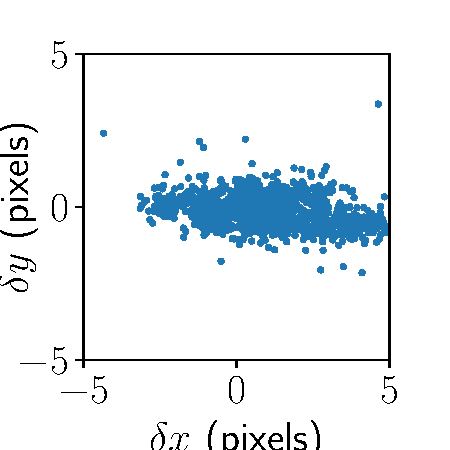
\includegraphics[width=\linewidth]{alignment-result-vectra-big-4.pdf}
		\caption{}
		\label{fig:alignmentresultbig4}
	\end{subfigure}
	\begin{subfigure}{0.24\linewidth}
		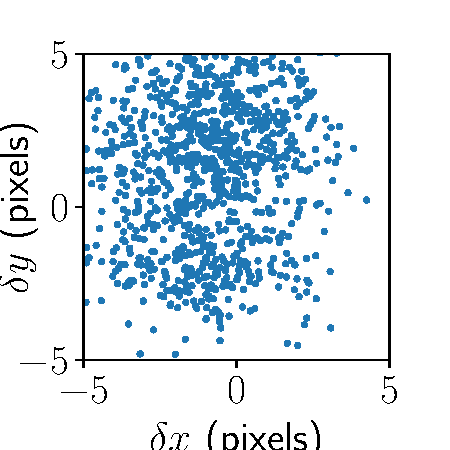
\includegraphics[width=\linewidth]{alignment-result-vectra-big-3.pdf}
		\caption{}
		\label{fig:alignmentresultbig3}
	\end{subfigure}
	\begin{subfigure}{0.24\linewidth}
		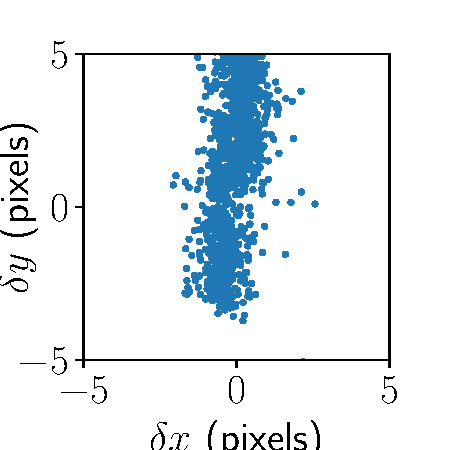
\includegraphics[width=\linewidth]{alignment-result-vectra-big-2.pdf}
		\caption{}
		\label{fig:alignmentresultbig2}
	\end{subfigure}
	\begin{subfigure}{0.24\linewidth}
		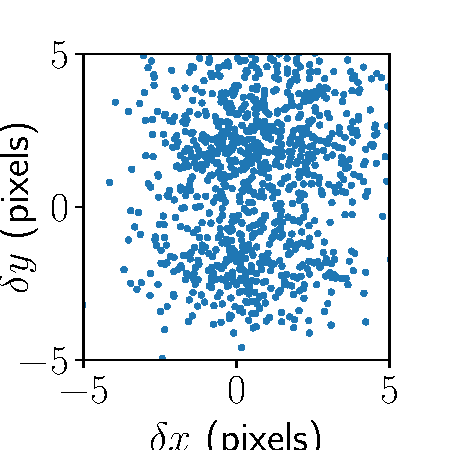
\includegraphics[width=\linewidth]{alignment-result-vectra-big-1.pdf}
		\caption{}
		\label{fig:alignmentresultbig1}
	\end{subfigure}
	\begin{subfigure}{0.24\linewidth}
		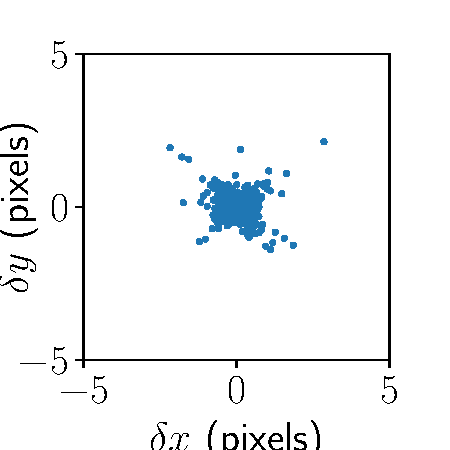
\includegraphics[width=\linewidth]{stitch-result-vectra-big-4.pdf}
		\caption{}
		\label{fig:stitchresultbig4}
	\end{subfigure}
	\begin{subfigure}{0.24\linewidth}
		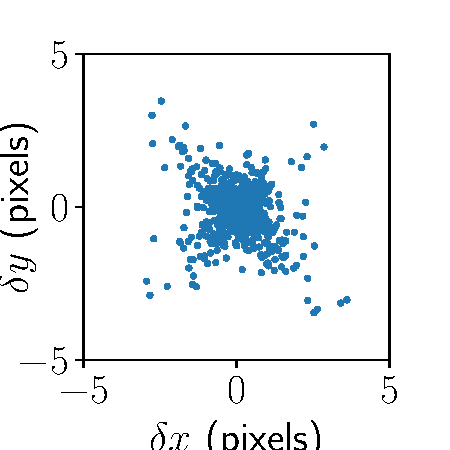
\includegraphics[width=\linewidth]{stitch-result-vectra-big-3.pdf}
		\caption{}
		\label{fig:stitchresultbig3}
	\end{subfigure}
	\begin{subfigure}{0.24\linewidth}
		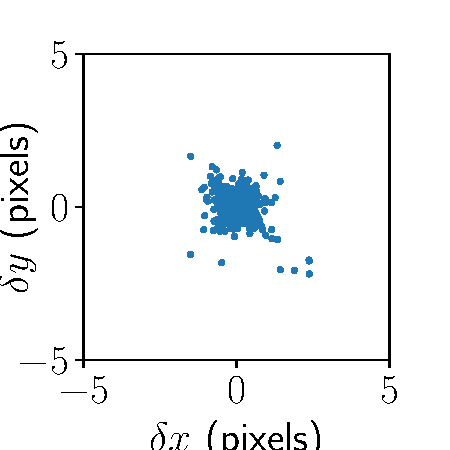
\includegraphics[width=\linewidth]{stitch-result-vectra-big-2.pdf}
		\caption{}
		\label{fig:stitchresultbig2}
	\end{subfigure}
	\begin{subfigure}{0.24\linewidth}
		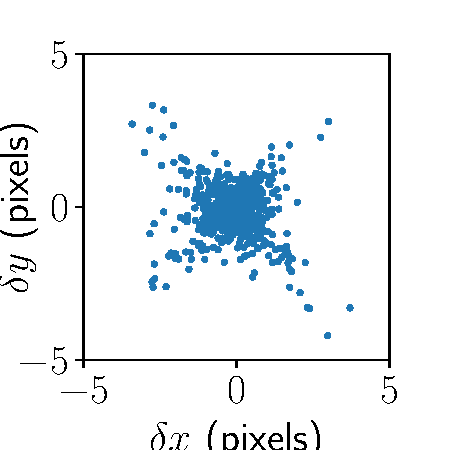
\includegraphics[width=\linewidth]{stitch-result-vectra-big-1.pdf}
		\caption{}
		\label{fig:stitchresultbig1}
	\end{subfigure}
	\caption{Distributions of $\delta\vec{r}_o$ for the overlaps in a larger image, code name \M11, taken with the Vectra 3.0 microscope.  The plots show overlaps between one field and the field \subref{fig:alignmentresultbig4} to its right, \subref{fig:alignmentresultbig3} under it and to the right, \subref{fig:alignmentresultbig2} under it, and \subref{fig:alignmentresultbig1} under it and to the left.  Each point indicates a single overlap.  Error bars are omitted because of the larger number of overlaps in this image.  \subref{fig:stitchresultbig4}--\subref{fig:stitchresultbig1} The same distributions for the respective overlap directions after stitching has been performed.}
	\label{fig:alignmentresultsbig}
\end{figure}

\Cref{fig:alignmentresultsbig} shows the same distributions for a larger image taken with the same microscope.  It shows similar effects, though they are harder to see due to the larger number of overlaps ($4527$ instead of $109$).  From these plots, it appears that although most fields are aligned well, there are a few outliers.  Furthermore, most of the outliers are corner overlaps (\cref{fig:stitchresultbig3,fig:stitchresultbig1}) and are misaligned in a diagonal direction.  Because there are no such effects in the edge overlaps (\cref{fig:stitchresultbig4,fig:stitchresultbig2}), the most likely explanation for the discrepancy between the individual alignment and the stitched alignment is that those particular corner overlaps are aligned badly.  The error estimation procedure correctly assigns a large error to them, and so they are weighted down in the final fit.

\clearpage

\subsubsection{JHU Vectra Polaris}

\Cref{fig:alignmentresultsJHUPolaris} shows the alignment movements from the \texttt{PZ1} sample.

The effects are smaller than the ones seen in the Vectra 3.0 microscope shown in \cref{fig:alignmentresults,fig:alignmentresultsbig} and are corrected by the stitching, as shown in the bottom row.  Some apparently badly-aligned overlaps form an X shape in the bottom row of plots, but as in the case of the \cref{fig:alignmentresultsbig}, these are mostly limited to corner overlaps and seem not to have a large effect on the overall alignment.

\begin{figure}[ht]
	\centering
	\begin{subfigure}{0.24\linewidth}
		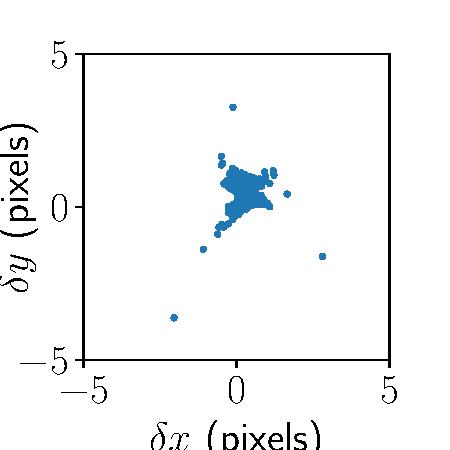
\includegraphics[width=\linewidth]{alignment-result-JHUPolaris-4.pdf}
		\caption{}
		\label{fig:alignmentresultJHUPolaris4}
	\end{subfigure}
	\begin{subfigure}{0.24\linewidth}
		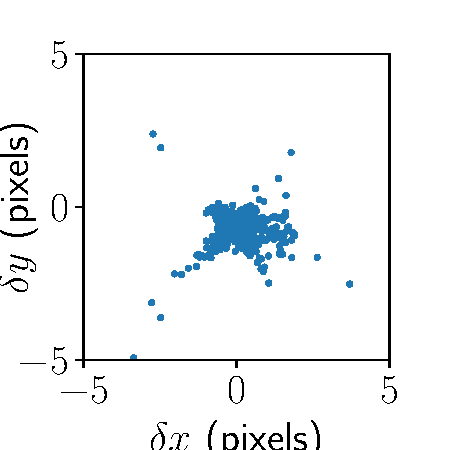
\includegraphics[width=\linewidth]{alignment-result-JHUPolaris-3.pdf}
		\caption{}
		\label{fig:alignmentresultJHUPolaris3}
	\end{subfigure}
	\begin{subfigure}{0.24\linewidth}
		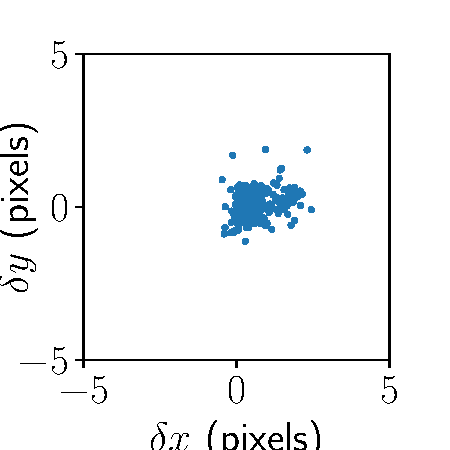
\includegraphics[width=\linewidth]{alignment-result-JHUPolaris-2.pdf}
		\caption{}
		\label{fig:alignmentresultJHUPolaris2}
	\end{subfigure}
	\begin{subfigure}{0.24\linewidth}
		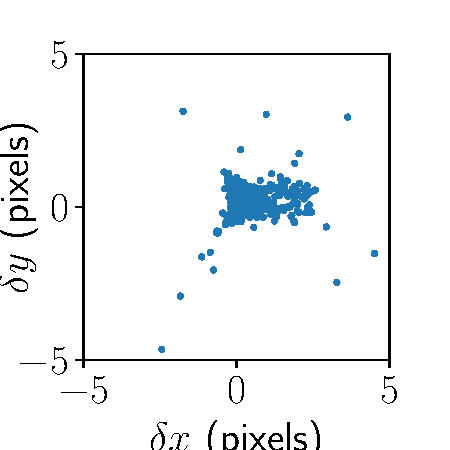
\includegraphics[width=\linewidth]{alignment-result-JHUPolaris-1.pdf}
		\caption{}
		\label{fig:alignmentresultJHUPolaris1}
	\end{subfigure}
	\begin{subfigure}{0.24\linewidth}
		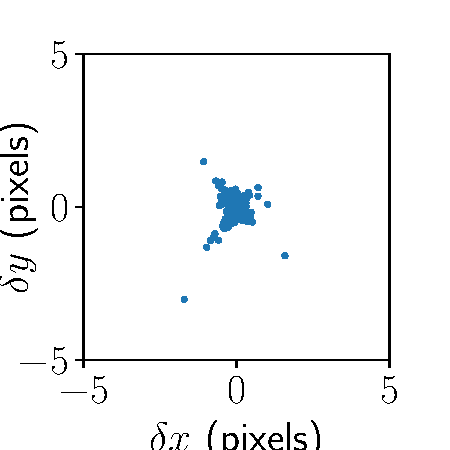
\includegraphics[width=\linewidth]{stitch-result-JHUPolaris-4.pdf}
		\caption{}
		\label{fig:stitchresultJHUPolaris4}
	\end{subfigure}
	\begin{subfigure}{0.24\linewidth}
		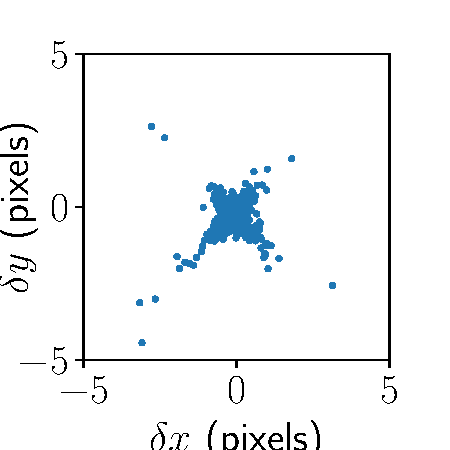
\includegraphics[width=\linewidth]{stitch-result-JHUPolaris-3.pdf}
		\caption{}
		\label{fig:stitchresultJHUPolaris3}
	\end{subfigure}
	\begin{subfigure}{0.24\linewidth}
		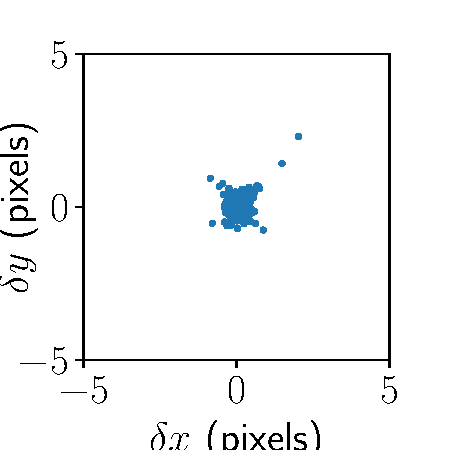
\includegraphics[width=\linewidth]{stitch-result-JHUPolaris-2.pdf}
		\caption{}
		\label{fig:stitchresultJHUPolaris2}
	\end{subfigure}
	\begin{subfigure}{0.24\linewidth}
		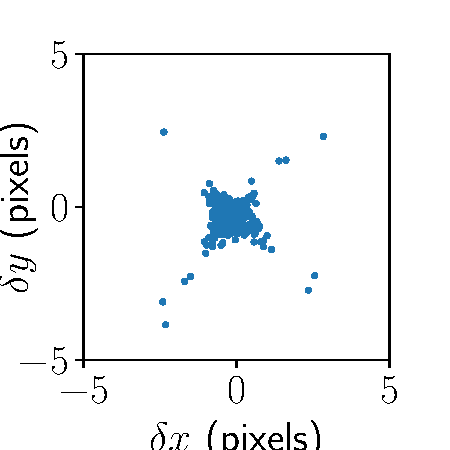
\includegraphics[width=\linewidth]{stitch-result-JHUPolaris-1.pdf}
		\caption{}
		\label{fig:stitchresultJHUPolaris1}
	\end{subfigure}
	\caption{Distributions of $\delta\vec{r}_o$ for the overlaps in an image, code name \texttt{PZ1}, taken with the JHU Vectra Polaris microscope.  The plots show overlaps between one field and the field \subref{fig:alignmentresultJHUPolaris4} to its right, \subref{fig:alignmentresultJHUPolaris3} under it and to the right, \subref{fig:alignmentresultJHUPolaris2} under it, and \subref{fig:alignmentresultJHUPolaris1} under it and to the left.  Each point indicates a single overlap.  Error bars are omitted because of the larger number of overlaps in this image.  \subref{fig:stitchresultJHUPolaris4}--\subref{fig:stitchresultJHUPolaris1} The same distributions for the respective overlap directions after stitching has been performed.}
	\label{fig:alignmentresultsJHUPolaris}
\end{figure}

\subsubsection{BMS Vectra Polaris}

\Cref{fig:alignmentresultsBMS} shows the alignment movements from the \texttt{ML1603480\_BMS078\_5\_22} sample.  The stitching gives a tighter distribution in the bottom row of plots than in the top row.

\begin{figure}[ht]
	\centering
	\begin{subfigure}{0.24\linewidth}
		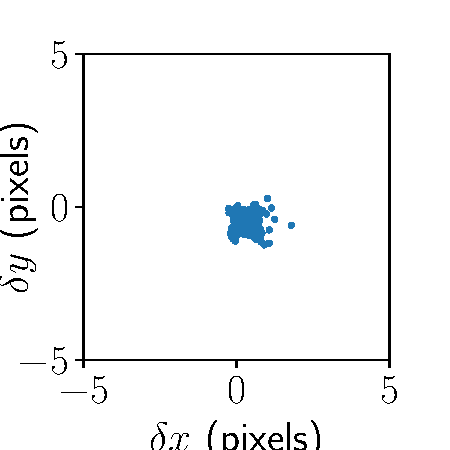
\includegraphics[width=\linewidth]{alignment-result-BMS-4.pdf}
		\caption{}
		\label{fig:alignmentresultBMS4}
	\end{subfigure}
	\begin{subfigure}{0.24\linewidth}
		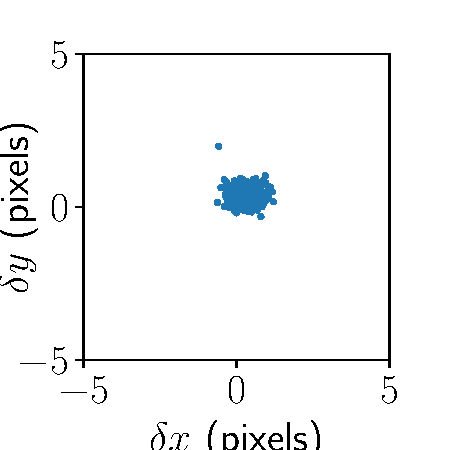
\includegraphics[width=\linewidth]{alignment-result-BMS-3.pdf}
		\caption{}
		\label{fig:alignmentresultBMS3}
	\end{subfigure}
	\begin{subfigure}{0.24\linewidth}
		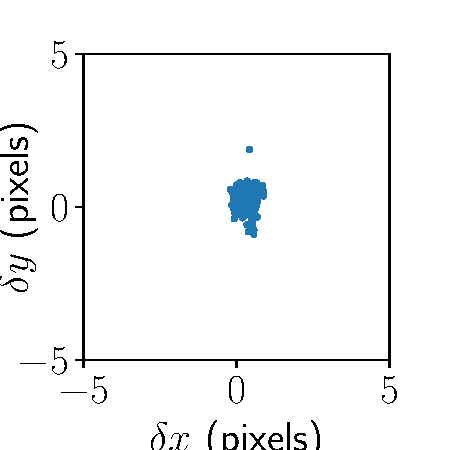
\includegraphics[width=\linewidth]{alignment-result-BMS-2.pdf}
		\caption{}
		\label{fig:alignmentresultBMS2}
	\end{subfigure}
	\begin{subfigure}{0.24\linewidth}
		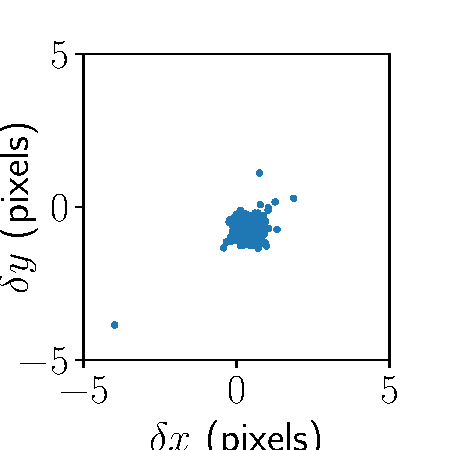
\includegraphics[width=\linewidth]{alignment-result-BMS-1.pdf}
		\caption{}
		\label{fig:alignmentresultBMS1}
	\end{subfigure}
	\begin{subfigure}{0.24\linewidth}
		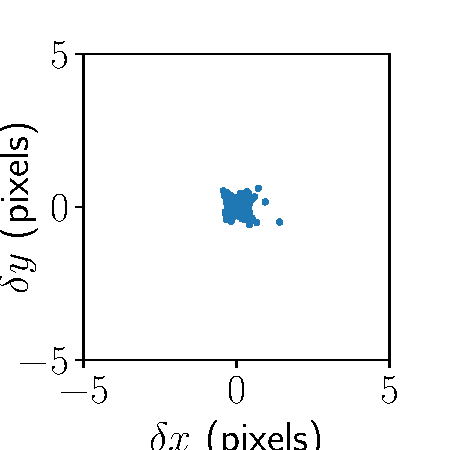
\includegraphics[width=\linewidth]{stitch-result-BMS-4.pdf}
		\caption{}
		\label{fig:stitchresultBMS4}
	\end{subfigure}
	\begin{subfigure}{0.24\linewidth}
		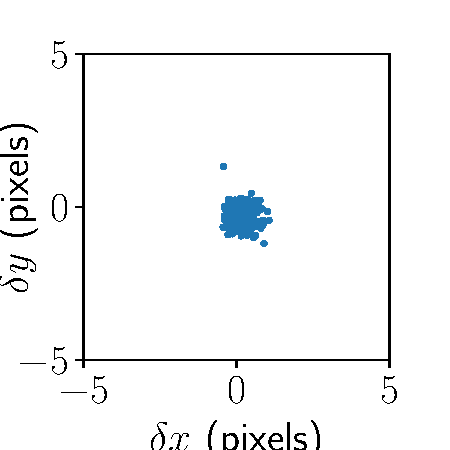
\includegraphics[width=\linewidth]{stitch-result-BMS-3.pdf}
		\caption{}
		\label{fig:stitchresultBMS3}
	\end{subfigure}
	\begin{subfigure}{0.24\linewidth}
		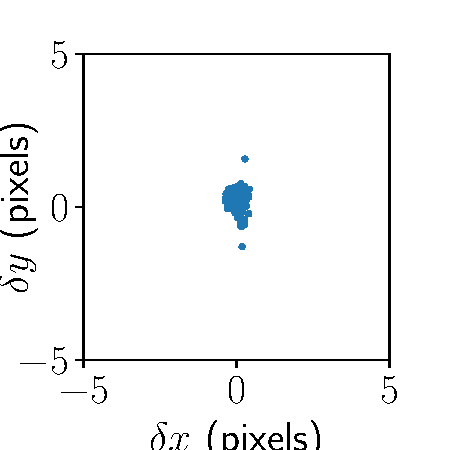
\includegraphics[width=\linewidth]{stitch-result-BMS-2.pdf}
		\caption{}
		\label{fig:stitchresultBMS2}
	\end{subfigure}
	\begin{subfigure}{0.24\linewidth}
		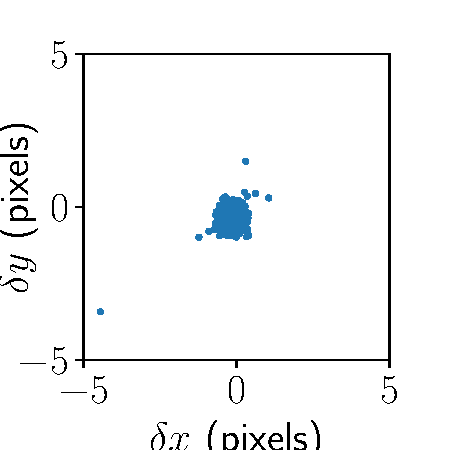
\includegraphics[width=\linewidth]{stitch-result-BMS-1.pdf}
		\caption{}
		\label{fig:stitchresultBMS1}
	\end{subfigure}
	\caption{Distributions of $\delta\vec{r}_o$ for the overlaps in an image, code name \texttt{TS19\_0181\_A\_1\_3\_BMS\_MITRE}, taken with the BMS Vectra Polaris microscope.  The plots show overlaps between one field and the field \subref{fig:alignmentresultBMS4} to its right, \subref{fig:alignmentresultBMS3} under it and to the right, \subref{fig:alignmentresultBMS2} under it, and \subref{fig:alignmentresultBMS1} under it and to the left.  Each point indicates a single overlap.  Error bars are omitted because of the larger number of overlaps in this image.  \subref{fig:stitchresultBMS4}--\subref{fig:stitchresultBMS1} The same distributions for the respective overlap directions after stitching has been performed.}
	\label{fig:alignmentresultsBMS}
\end{figure}

\subsubsection{Akoya Vectra Polaris}

\Cref{fig:alignmentresultsAKY} shows the alignment movements from the \texttt{TS19\_0181\_A\_1\_3\_BMS\_MITRE} sample.

All four of the plots in the top row show two clusters of overlaps, indicating that there are systematic effects present in addition to the random movement.  \Cref{sec:AKY2D} will investigate those effects in greater detail.

\begin{figure}[ht]
	\centering
	\begin{subfigure}{0.24\linewidth}
		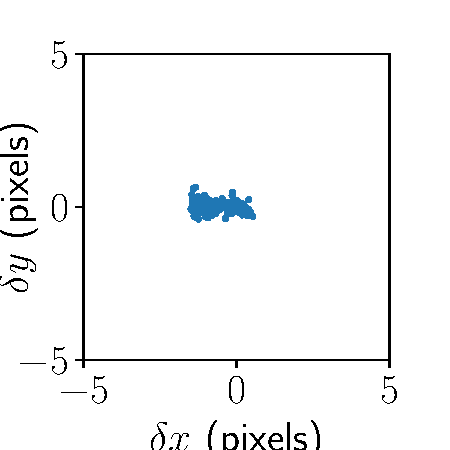
\includegraphics[width=\linewidth]{alignment-result-AKY-4.pdf}
		\caption{}
		\label{fig:alignmentresultAKY4}
	\end{subfigure}
	\begin{subfigure}{0.24\linewidth}
		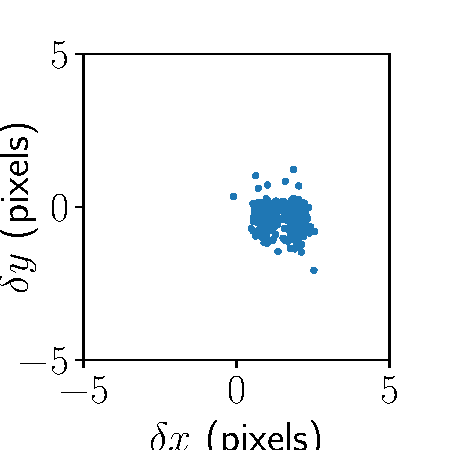
\includegraphics[width=\linewidth]{alignment-result-AKY-3.pdf}
		\caption{}
		\label{fig:alignmentresultAKY3}
	\end{subfigure}
	\begin{subfigure}{0.24\linewidth}
		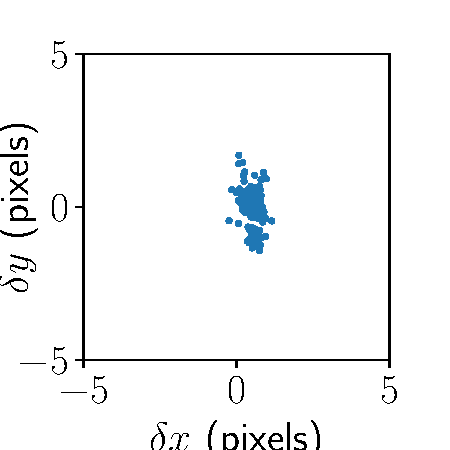
\includegraphics[width=\linewidth]{alignment-result-AKY-2.pdf}
		\caption{}
		\label{fig:alignmentresultAKY2}
	\end{subfigure}
	\begin{subfigure}{0.24\linewidth}
		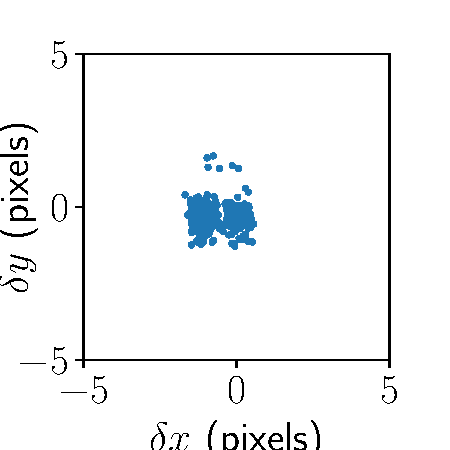
\includegraphics[width=\linewidth]{alignment-result-AKY-1.pdf}
		\caption{}
		\label{fig:alignmentresultAKY1}
	\end{subfigure}
	\begin{subfigure}{0.24\linewidth}
		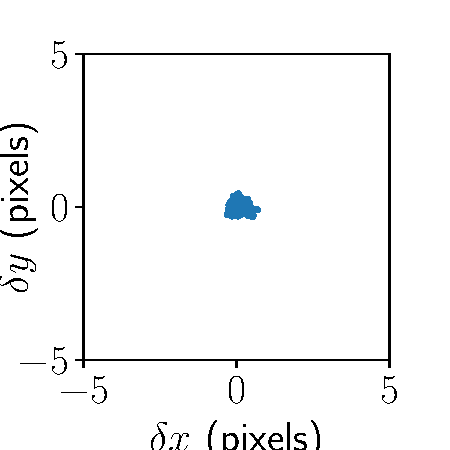
\includegraphics[width=\linewidth]{stitch-result-AKY-4.pdf}
		\caption{}
		\label{fig:stitchresultAKY4}
	\end{subfigure}
	\begin{subfigure}{0.24\linewidth}
		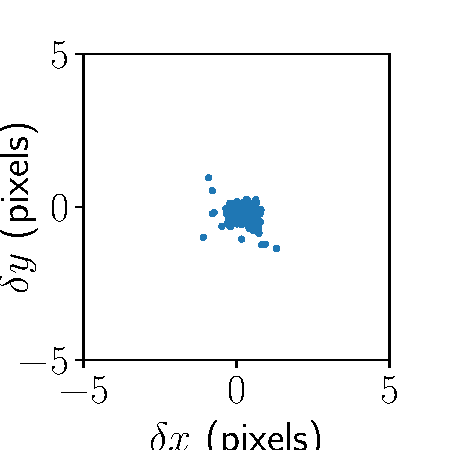
\includegraphics[width=\linewidth]{stitch-result-AKY-3.pdf}
		\caption{}
		\label{fig:stitchresultAKY3}
	\end{subfigure}
	\begin{subfigure}{0.24\linewidth}
		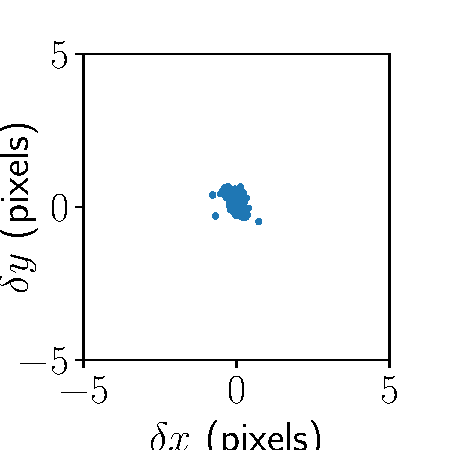
\includegraphics[width=\linewidth]{stitch-result-AKY-2.pdf}
		\caption{}
		\label{fig:stitchresultAKY2}
	\end{subfigure}
	\begin{subfigure}{0.24\linewidth}
		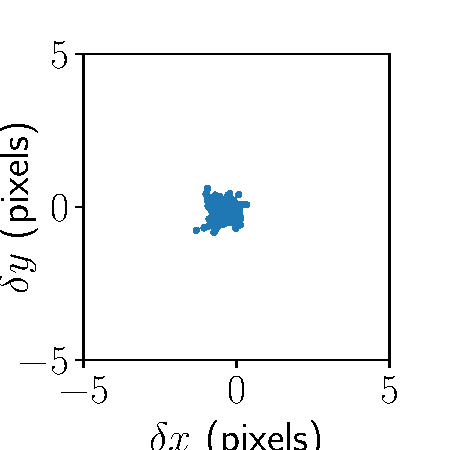
\includegraphics[width=\linewidth]{stitch-result-AKY-1.pdf}
		\caption{}
		\label{fig:stitchresultAKY1}
	\end{subfigure}
	\caption{Distributions of $\delta\vec{r}_o$ for the overlaps in an image, code name \texttt{TS19\_0181\_A\_1\_3\_BMS\_MITRE}, taken with Akoya's Vectra Polaris microscope.  The plots show overlaps between one field and the field \subref{fig:alignmentresultAKY4} to its right, \subref{fig:alignmentresultAKY3} under it and to the right, \subref{fig:alignmentresultAKY2} under it, and \subref{fig:alignmentresultAKY1} under it and to the left.  Each point indicates a single overlap.  Error bars are omitted because of the larger number of overlaps in this image.  \subref{fig:stitchresultAKY4}--\subref{fig:stitchresultAKY1} The same distributions for the respective overlap directions after stitching has been performed.}
	\label{fig:alignmentresultsAKY}
\end{figure}

\clearpage

\subsection{Consistency of the errors}
\label{sec:pulls}

We also want to ensure that our estimate of the errors on the alignment are correct.  To do this, we use what is known as a ``pull'' distribution.  The idea is to find a quantity $x$ that we expect to be $0$.  Any actual measurement of $x$ will not necessarily be $0$, but we perform multiple measurements $x_i$, we expect to end up with a normal distribution centered at $0$ and with a width of $\sigma$.  If we instead look at the distribution of $x_i/\sigma$, the width of the normal distribution will be $1$.

In general, we do not know $\sigma$ in advance, but we have an estimate $\sigma_i$ of the error on each individual measurement.  The idea of a pull distribution is that we plot $x_i/\sigma_i$ and look at the width of the resulting distribution.  If it is close to $1$, that indicates that our error estimate was correct.

\subsubsection{JHU Vectra 3.0}

\Cref{fig:squarepulls} shows the pull distributions for the total displacement from pairwise alignments for moving around in a square or diamond.  For a perfect alignment, this quantity would be $0$, so it is a good candidate for a pull distribution.  As the figures show, the standard deviations of all pull distributions are close to $1$, indicating that our error estimates for both edge and corner overlaps are reasonable.

\begin{figure}[ht]
	\centering
	\begin{subfigure}{0.32\linewidth}
		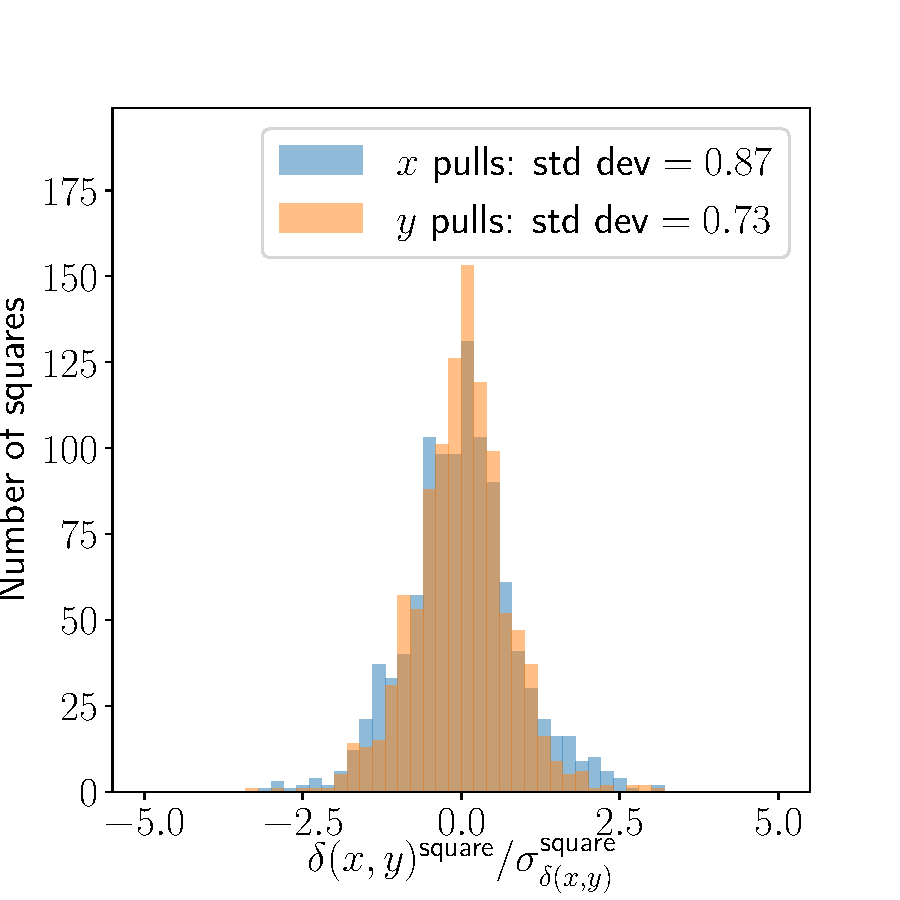
\includegraphics[width=\linewidth]{squarepull1.pdf}
		\caption{}
		\label{fig:squarepull1}
	\end{subfigure}
	\begin{subfigure}{0.32\linewidth}
		\includegraphics[width=\linewidth]{squarepull2.pdf}
		\caption{}
		\label{fig:squarepull2}
	\end{subfigure}
	\begin{subfigure}{0.32\linewidth}
		\includegraphics[width=\linewidth]{squarepulldiagram.pdf}
		\caption{}
		\label{fig:squarepulldiagram}
	\end{subfigure}
	\begin{subfigure}{0.32\linewidth}
		\includegraphics[width=\linewidth]{diamondpull1.pdf}
		\caption{}
		\label{fig:diamondpull1}
	\end{subfigure}
	\begin{subfigure}{0.32\linewidth}
		\includegraphics[width=\linewidth]{diamondpull2.pdf}
		\caption{}
		\label{fig:diamondpull2}
	\end{subfigure}
	\begin{subfigure}{0.32\linewidth}
		\includegraphics[width=\linewidth]{diamondpulldiagram.pdf}
		\caption{}
		\label{fig:diamondpulldiagram}
	\end{subfigure}
	\caption{\subref{fig:squarepull1}, \subref{fig:squarepull2} The pull distributions in $x$ and $y$ for the total displacement obtained from pairwise alignment when moving around in a square, as shown in \subref{fig:squarepulldiagram}, for two different images, code names \M11 and \M23, respectively, collected with the Vectra 3.0 microscope.  \subref{fig:diamondpull1}, \subref{fig:diamondpull2} The corresponding pull distributions for those two datasets when moving in a diamond, as shown in \subref{fig:diamondpulldiagram}.}
	\label{fig:squarepulls}
\end{figure}

\Cref{fig:stitchpulls} shows a different metric for our error estimation.  In these plots, we calculate the misalignment for each overlapping pair of fields after stitching, as in \cref{fig:stitchresult1,fig:stitchresult2,fig:stitchresult3,fig:stitchresult4}, and create pull distributions for the $x$ and $y$ resdiuals.  Again, the standard deviations of the pull distributions are close to $1$.

\begin{figure}[ht]
	\centering
	\begin{subfigure}{0.24\linewidth}
		\includegraphics[width=\linewidth]{stitch-pull-4-1.pdf}
		\caption{}
		\label{fig:stitchpull41}
	\end{subfigure}
	\begin{subfigure}{0.24\linewidth}
		\includegraphics[width=\linewidth]{stitch-pull-3-1.pdf}
		\caption{}
		\label{fig:stitchpull31}
	\end{subfigure}
	\begin{subfigure}{0.24\linewidth}
		\includegraphics[width=\linewidth]{stitch-pull-2-1.pdf}
		\caption{}
		\label{fig:stitchpull21}
	\end{subfigure}
	\begin{subfigure}{0.24\linewidth}
		\includegraphics[width=\linewidth]{stitch-pull-1-1.pdf}
		\caption{}
		\label{fig:stitchpull11}
	\end{subfigure}
	\begin{subfigure}{0.24\linewidth}
		\includegraphics[width=\linewidth]{stitch-pull-4-2.pdf}
		\caption{}
		\label{fig:stitchpull42}
	\end{subfigure}
	\begin{subfigure}{0.24\linewidth}
		\includegraphics[width=\linewidth]{stitch-pull-3-2.pdf}
		\caption{}
		\label{fig:stitchpull32}
	\end{subfigure}
	\begin{subfigure}{0.24\linewidth}
		\includegraphics[width=\linewidth]{stitch-pull-2-2.pdf}
		\caption{}
		\label{fig:stitchpull22}
	\end{subfigure}
	\begin{subfigure}{0.24\linewidth}
		\includegraphics[width=\linewidth]{stitch-pull-1-2.pdf}
		\caption{}
		\label{fig:stitchpull12}
	\end{subfigure}
	\caption{Pull distributions in $x$ and $y$ for the residual pairwise misalignment after stitching, as shown in \cref{fig:stitchresult4,fig:stitchresult3,fig:stitchresult2,fig:stitchresult1}, for two different images, \M11 and \M23, collected with the Vectra 3.0 microscope.  The plots show distributions for overlaps between one field and the field \subref{fig:stitchpull41}, \subref{fig:stitchpull42} to its right, \subref{fig:stitchpull31}, \subref{fig:stitchpull32} under it and to the right, \subref{fig:stitchpull21}, \subref{fig:stitchpull22}  under it, and \subref{fig:stitchpull11}, \subref{fig:stitchpull12}  under it and to the left.}
	\label{fig:stitchpulls}
\end{figure}

The standard deviations of the pull distributions were used to determine the factor of $1/16$ used to correct \cref{eq:overlapcovariance} to \cref{eq:overlapcovariancecorrected}.  The fact that, after making this correction, the standard deviations are $1$ for multiple different images as well as for pull distributions of two different quantities lends confidence to the \emph{method} of error estimation.  Remaining deviations from $1$ indicate that there is still some amount of room for improvement.

\clearpage

\subsection{Linear transformation matrix}

As described in \cref{sec:stitching}, when we stitch the alignment we also obtain the linear matrix $\matrixbold{A}$, which describes the relationship between the distance that the microscope is supposed to move $\Delta\vec{r}$ and the average distance it actually moves $\matrixbold{A}\Delta\vec{r}$.  We expect it to be more or less constant for different images taken with the same microscope, although of course the mechanical parts can also degrade over time, change due to maintenance, or be replaced.

The primary purpose of the alignment and stitching is to determine the relative locations of the high-powered fields, and when only a single island is present $\matrixbold{A}$ is not necessary for this purpose.  When there are multiple islands, as in \cref{fig:islands}, including $\matrixbold{A}$ in the fit allows us to obtain those islands' approximate relative locations.  In either case, we do not need the precise values of $\matrixbold{A}$'s entries for any analysis, but the matrix still provides interesting information about the mechanical calibration of the microscope.

\subsubsection{JHU Vectra 3.0}

For the \M11 dataset, we find
\begin{align}
\matrixbold{A}=&\begin{pmatrix}
\num{0.999132\pm.000009} &
\num{.000173\pm.000013} \\
\num{0.000103\pm.000010} &
\num{0.998652\pm.000014}
\end{pmatrix} \\
=\matrixbold{I} + &\begin{pmatrix}
\num{-0.868\pm.009} &
\num{.173\pm.013} \\
\num{0.103\pm.010} &
\num{-1.348\pm.014}
\end{pmatrix} \times \num{e-3}
\label{eq:Amatrix_M11}
\end{align}
The Vectra 3.0 scans fields of size $1344\times1004$ $\text{pixels}^2$.  The entries of $\matrixbold{A}$ tell us that on average, when moving one field to the right, the microscope ends up $0.9$ pixels to the left and $0.1$ pixels below where it should, and when moving down, it ends up $0.1$ pixels to the right and $1.1$ pixels above where it should.  Although the top row of \cref{fig:alignmentresults} shows that the random scatter is a larger effect, the average shift is noticeable.

\subsubsection{JHU Vectra Polaris}

From the sample named \texttt{PZ1}, we find the linear transformation matrix to be
\begin{align}
\matrixbold{A}=&\begin{pmatrix}
\num{0.999782(4)} &
\num{-0.000308(5)} \\
\num{-0.000327(4)} &
\num{0.999994(5)}
\end{pmatrix} \\
=\matrixbold{I} + &\begin{pmatrix}
\num{-0.218(4)} &
\num{-0.308(5)} \\
\num{-0.327(4)} &
\num{-0.006(5)}
\end{pmatrix} \times \num{e-3}
\label{eq:Amatrix_PZ1}
\end{align}
The Vectra Polaris scans fields of size $1876\times1404$ $\text{pixels}^2$, slightly larger than the Vectra 3.0.  The result is that when moving one field to the right, the microscope undershoots by an average of $0.3$ pixels and moves up by $0.5$ pixels.  When moving down, it moves to the right by an average of $0.3$ pixels.

\subsubsection{BMS Vectra Polaris}

From the sample named \texttt{ML1603480\_BMS078\_5\_22}, we find the linear transformation matrix to be
\begin{align}
\matrixbold{A}=&\begin{pmatrix}
\num{0.9998290(35)} &
\num{-0.000253(4)} \\
\num{0.000364(4)} &
\num{0.999904(5)}
\end{pmatrix} \\
=\matrixbold{I} + &\begin{pmatrix}
\num{-0.1710(35)} &
\num{-0.253(4)} \\
\num{0.364(4)} &
\num{-0.096(5)}
\end{pmatrix} \times \num{e-3}
\label{eq:Amatrix_ML1603474_BMS069_5_21}
\end{align}
When moving one field to the right, the microscope undershoots by an average of $0.2$ pixels and also moves down by $0.5$ pixels.  When moving down, it undershoots by an average of $0.1$ pixels and moves to the left by $0.3$ pixels.

\subsubsection{Akoya Vectra Polaris}

From the sample named \texttt{TS19\_0181\_A\_1\_3\_BMS\_MITRE}, we find the linear transformation matrix to be
\begin{align}
\matrixbold{A}=&\begin{pmatrix}
\num{1.000503(5)} &
\num{-0.000454(5)} \\ 
\num{2.44(31)e-05} &
\num{1.000044(4)}
\end{pmatrix} \\
=\matrixbold{I} + &\begin{pmatrix}
\num{0.503(5)} &
\num{-0.454(5)} \\
\num{0.0244(31)} &
\num{0.044(4)}
\end{pmatrix} \times \num{e-3}
\label{eq:Amatrix_TS18_0541_BMS_MITRE}
\end{align}
When moving one field to the right, the microscope overshoots by an average of $0.7$ pixels, as expected from \cref{fig:alignmentresultAKY4}, and when moving down, it ends up $0.5$ pixels to the left of the desired location, as expected from \cref{fig:alignmentresultAKY2}.

\clearpage

\subsection{Two-dimensional dependence of shifts}

Finally, we can plot the movements of each field in the image.  These plots give a full picture of the alignment in all of its detail, and will shed more light on the features observed in the previous sections.

In these plots, we show $\vec{r}_k-\matrixbold{A}\vec{r}_k^n$, subtracting the effect of the affine matrix $\matrixbold{A}$.  In this way, we measure the random shifts as well as systematic effects not described by the affine matrix.  Each field is assigned a color in $x$ and $y$ based on the size of the alignment shift.

For each individual microscope, the color scales for $x$ and $y$ are set to be the same.  However, we do not set those scales to be the same between all microscopes because the sizes of the relevant shifts are different for each one, as will be immediately clear from the plots.

\subsubsection{JHU Vectra 3.0}
\label{sec:vectra2D}

\Cref{fig:2Dvectra} shows the two-dimensional distribution of the shifts for the \M11 dataset.  This plot highlights periodic features, with an amplitude of several pixels, in the 2D distribution.

\begin{figure}[ht]
	\centering
	\begin{subfigure}{0.49\linewidth}
		\includegraphics[width=\linewidth]{2D-shifts-JHUVectra-x}
		\caption{}
		\label{fig:2Dvectrax}
	\end{subfigure}
	\begin{subfigure}{0.49\linewidth}
		\includegraphics[width=\linewidth]{2D-shifts-JHUVectra-y}
		\caption{}
		\label{fig:2Dvectray}
	\end{subfigure}
	\caption{The shifts in \subref{fig:2Dvectrax} $x$ and \subref{fig:2Dvectray} $y$ for the fields in \M11.}
	\label{fig:2Dvectra}
\end{figure}

To analyze the sinusoidal pattern more quantitatively, we can project onto the x and y axes and make a profile plot.  Each point in \cref{fig:sinewavexx1} represents a column in \cref{fig:2Dvectrax}: the marker gives the average shift for that column and the error bar gives the standard deviation.  Similarly, each point and associated error bar of \cref{fig:sinewaveyy1} show the average and standard deviation of the shifts in the corresponding column of \cref{fig:2Dvectray}.  The points are fitted to a sine wave.

As a cross check, similar plots are also shown for a second dataset in \cref{fig:sinewavexx2,fig:sinewaveyy2}, and the amplitudes and wavelengths of the sine waves are in agreement between both datasets.  This indicates that the effect is probably a property of the microscope.  For instance, the cam wheels controlling the microscope movement may have a slight eccentricity instead of being exactly circular.

\begin{figure}[ht]
	\centering
	\begin{subfigure}{0.24\linewidth}
	       \includegraphics[width=\linewidth]{sine-wave-xx-1.pdf}
	       \caption{}
	       \label{fig:sinewavexx1}
	\end{subfigure}
	\begin{subfigure}{0.24\linewidth}
	       \includegraphics[width=\linewidth]{sine-wave-yy-1.pdf}
	       \caption{}
	       \label{fig:sinewaveyy1}
	\end{subfigure}
	\begin{subfigure}{0.24\linewidth}
	       \includegraphics[width=\linewidth]{sine-wave-xx-2.pdf}
	       \caption{}
	       \label{fig:sinewavexx2}
	\end{subfigure}
	\begin{subfigure}{0.24\linewidth}
	       \includegraphics[width=\linewidth]{sine-wave-yy-2.pdf}
	       \caption{}
	       \label{fig:sinewaveyy2}
	\end{subfigure}
	\caption{Profile plot of the measured alignment shifts for overlaps in a particular row or column.  Each data point shows the average shift for the row or column, and the error bars show the standard deviation.  \subref{fig:sinewavexx1} shows shifts in the $x$ direction as a function of $x$ and \subref{fig:sinewaveyy1} shows shifts in the $y$ direction as a function of $y$, both for the \M11 dataset.  \subref{fig:sinewavexx2} and \subref{fig:sinewaveyy2} show the same for the \M23 dataset.  The plots are fitted to a sine curve, whose amplitude and wavelength are indicated on the plot.}
	\label{fig:sinewaves}
       
\end{figure}

\subsubsection{JHU Vectra Polaris}
\label{sec:polaris2D}

\Cref{fig:2Dpolaris} shows the two-dimensional distribution of the shifts for the \texttt{PZ1} dataset.  This plot shows that at the beginning of the scan, the microscope took some time to gradually ``settle in'' to its final position.  The alignment procedure accounts for this settling.

\begin{figure}[ht]
	\centering
	\begin{subfigure}{0.49\linewidth}
		\includegraphics[width=\linewidth]{2D-shifts-JHUPolaris-x}
		\caption{}
		\label{fig:2Dpolarisx}
	\end{subfigure}
	\begin{subfigure}{0.49\linewidth}
		\includegraphics[width=\linewidth]{2D-shifts-JHUPolaris-y}
		\caption{}
		\label{fig:2Dpolarisy}
	\end{subfigure}
	\caption{The shifts in \subref{fig:2Dpolarisx} $x$ and \subref{fig:2Dpolarisy} $y$ for the fields in \texttt{PZ1}.}
	\label{fig:2Dpolaris}
\end{figure}

\subsubsection{BMS Vectra Polaris}
\label{sec:BMS2D}

\Cref{fig:2DBMS} shows the two-dimensional distribution of the shifts for the \texttt{ML1603480\_BMS078\_5\_22} dataset.  This dataset is very stable and only contains some seemingly random noise, all less than one pixel.

\begin{figure}[ht]
	\centering
	\begin{subfigure}{0.49\linewidth}
		\includegraphics[width=\linewidth]{2D-shifts-BMS-x}
		\caption{}
		\label{fig:2DBMSx}
	\end{subfigure}
	\begin{subfigure}{0.49\linewidth}
		\includegraphics[width=\linewidth]{2D-shifts-BMS-y}
		\caption{}
		\label{fig:2DBMSy}
	\end{subfigure}
	\caption{The shifts in \subref{fig:2DBMSx} $x$ and \subref{fig:2DBMSy} $y$ for the fields in \texttt{ML1603480\_BMS078\_5\_22}.}
	\label{fig:2DBMS}
\end{figure}

\Cref{fig:2DBMSbad} shows the two-dimensional distribution of the shifts for the \texttt{ML1603474\_BMS069\_5\_21} dataset, a different image taking with the same microscope.  The most striking feature of this plot is that the microscope apparently jumped to the left by $10$ pixels in $x$ for several rows in the middle of the scan, then jumped again by $30$ pixels to the right, then moved back closer to its original position.  This kind of shift most likely only happens occasionally, but can severely degrade data quality if left uncorrected.

\begin{figure}[ht]
	\centering
	\begin{subfigure}{0.49\linewidth}
		\includegraphics[width=\linewidth]{2D-shifts-BMS2-x}
		\caption{}
		\label{fig:2DBMSbadx}
	\end{subfigure}
	\begin{subfigure}{0.49\linewidth}
		\includegraphics[width=\linewidth]{2D-shifts-BMS2-y}
		\caption{}
		\label{fig:2DBMSbady}
	\end{subfigure}
	\caption{The shifts in \subref{fig:2DBMSbadx} $x$ and \subref{fig:2DBMSbady} $y$ for the fields in \texttt{ML1603474\_BMS069\_5\_21}.}
	\label{fig:2DBMSbad}
\end{figure}

\subsubsection{Akoya Vectra Polaris results}
\label{sec:AKY2D}

\Cref{fig:2DAKY} shows the two-dimensional distribution of the shifts for the \texttt{TS19\_0181\_A\_1\_3\_BMS\_MITRE} dataset.  This dataset is quite stable.   It shows a $1$-pixel settling effect at the beginning of the scan and periodic modulations with amplitudes of less than $1$ pixel.

\begin{figure}[ht]
	\centering
	\begin{subfigure}{0.49\linewidth}
		\includegraphics[width=\linewidth]{2D-shifts-AKY-x}
		\caption{}
		\label{fig:2DAKYx}
	\end{subfigure}
	\begin{subfigure}{0.49\linewidth}
		\includegraphics[width=\linewidth]{2D-shifts-AKY-y}
		\caption{}
		\label{fig:2DAKYy}
	\end{subfigure}
	\caption{The shifts in \subref{fig:2DAKYx} $x$ and \subref{fig:2DAKYy} $y$ for the fields in \texttt{TS19\_0181\_A\_1\_3\_BMS\_MITRE}.}
	\label{fig:2DAKY}
\end{figure}

\Cref{fig:sinewavesAKY} shows projections of these plots onto the $x$ and $y$ axes, which help to more quantitatively identify the periodic pattern.

\begin{figure}[ht]
	\centering
	\begin{subfigure}{0.49\linewidth}
		\includegraphics[width=\linewidth]{sine-wave-xx-AKY}
		\caption{}
		\label{fig:sinewavexxAKY}
	\end{subfigure}
	\begin{subfigure}{0.49\linewidth}
		\includegraphics[width=\linewidth]{sine-wave-yy-AKY}
		\caption{}
		\label{fig:sinewaveyyAKY}
	\end{subfigure}
	\caption{Profile plots of the measured alignment shifts for overlaps in a particular row or column.  Each data point shows the average shift for the row or column, and the error bars show the standard deviation.  \subref{fig:sinewavexx1} shows shifts in the $x$ direction as a function of $x$ and \subref{fig:sinewaveyy1} shows in the $y$ direction as a function of $y$, both for the \texttt{TS19\_0181\_A\_1\_3\_BMS\_MITRE} dataset.  \subref{fig:sinewavexx1} is fitted to a sine curve, whose amplitude and wavelength are indicated on the plot.}
	\label{fig:sinewavesAKY}
\end{figure}

\clearpage

\subsection{Isotropy of residual misalignments}

As \cref{fig:stitchresultbig4,fig:stitchresultbig3,fig:stitchresultbig2,fig:stitchresultbig1} show, the residual misalignments after stitching are not isotropic.  To some extent, this is to be expected, because the input to the alignment, the edges and corners, are not isotropic either.  Nevertheless, the lack of isotropy might indicate an imperfection in previous steps of the calibration (such as flatfielding or warping) or may come from an incorrect relative weight assigned to the edge and corner overlaps in the stitching procedure.  We can note that the pull distributions in \cref{sec:pulls} are generally wider for the corner overlaps than for the edge overlaps, lending some credence to this second possibility.

\subsubsection{JHU Vectra 3.0}

In \cref{fig:stitchfourierseries}, we attempt to quantify this anisotropy by producing a histogram of the angle $\phi$ of the overlaps in \cref{fig:stitchresultbig4,fig:stitchresultbig3,fig:stitchresultbig2,fig:stitchresultbig1}.  Each histogram is fitted to a Fourier series, and the first four terms are shown on the plot.  An isotropic distribution would produce flat histograms.

\begin{figure}[ht]
	\centering
	\begin{subfigure}{0.24\linewidth}
		\includegraphics[width=\linewidth]{isotropy-histogram-JHUVectra-4-all}
		\caption{}
		\label{fig:isotropyhistvectra4all}
	\end{subfigure}
	\begin{subfigure}{0.24\linewidth}
		\includegraphics[width=\linewidth]{isotropy-histogram-JHUVectra-3-all}
		\caption{}
		\label{fig:isotropyhistvectra3all}
	\end{subfigure}
	\begin{subfigure}{0.24\linewidth}
		\includegraphics[width=\linewidth]{isotropy-histogram-JHUVectra-2-all}
		\caption{}
		\label{fig:isotropyhistvectra2all}
	\end{subfigure}
	\begin{subfigure}{0.24\linewidth}
		\includegraphics[width=\linewidth]{isotropy-histogram-JHUVectra-1-all}
		\caption{}
		\label{fig:isotropyhistvectra1all}
	\end{subfigure}
	\begin{subfigure}{0.24\linewidth}
		\includegraphics[width=\linewidth]{isotropy-histogram-JHUVectra-4-edges}
		\caption{}
		\label{fig:isotropyhistvectra4edges}
	\end{subfigure}
	\begin{subfigure}{0.24\linewidth}
		\includegraphics[width=\linewidth]{isotropy-histogram-JHUVectra-3-edges}
		\caption{}
		\label{fig:isotropyhistvectra3edges}
	\end{subfigure}
	\begin{subfigure}{0.24\linewidth}
		\includegraphics[width=\linewidth]{isotropy-histogram-JHUVectra-2-edges}
		\caption{}
		\label{fig:isotropyhistvectra2edges}
	\end{subfigure}
	\begin{subfigure}{0.24\linewidth}
		\includegraphics[width=\linewidth]{isotropy-histogram-JHUVectra-1-edges}
		\caption{}
		\label{fig:isotropyhistvectra1edges}
	\end{subfigure}
	\begin{subfigure}{0.24\linewidth}
		\includegraphics[width=\linewidth]{isotropy-histogram-JHUVectra-4-corners}
		\caption{}
		\label{fig:isotropyhistvectra4corners}
	\end{subfigure}
	\begin{subfigure}{0.24\linewidth}
		\includegraphics[width=\linewidth]{isotropy-histogram-JHUVectra-3-corners}
		\caption{}
		\label{fig:isotropyhistvectra3corners}
	\end{subfigure}
	\begin{subfigure}{0.24\linewidth}
		\includegraphics[width=\linewidth]{isotropy-histogram-JHUVectra-2-corners}
		\caption{}
		\label{fig:isotropyhistvectra2corners}
	\end{subfigure}
	\begin{subfigure}{0.24\linewidth}
		\includegraphics[width=\linewidth]{isotropy-histogram-JHUVectra-1-corners}
		\caption{}
		\label{fig:isotropyhistvectra1corners}
	\end{subfigure}
	\caption{Distributions of the angles $\phi$ of the residual misalignments, after stitching, for the overlaps in the \M11 dataset, taken with the Vectra 3.0 microscope.  The plots show overlaps between one field and the field \subref{fig:isotropyhistvectra4all} to its right, \subref{fig:isotropyhistvectra3all} under it and to the right, \subref{fig:isotropyhistvectra2all} under it, and \subref{fig:isotropyhistvectra1all} under it and to the left.  The histograms count the number of overlaps, and the curves show the first few terms in the Fourier series.  \subref{fig:isotropyhistvectra4edges}--\subref{fig:isotropyhistvectra1edges} The same distributions when stitching using only edge overlaps.  \subref{fig:isotropyhistvectra4corners}--\subref{fig:isotropyhistvectra1corners} The same distributions when stitching using only corner overlaps.}
	\label{fig:stitchfourierseries}
\end{figure}

\section{Summary}

In this note, we describe the alignment and stitching of a microscope image composed of up to $1000$ fields.  Our procedure includes an estimation of the error on each field, which are propagated throughout the procedure to obtain a final error estimate and covariance matrix for the positions of the fields.  To demonstrate the method, we run it over several data samples collected by different microscopes.  \Cref{table:microscopes} compares the alignment behavior of the different microscopes used.  The method provided here, which runs in a few minutes, forms an important part of the data calibration in the astropath framework.

\begin{table}[ht]
	\centering
	\begin{tabular}{|l|c|c|c|c|c|}
	\hline
	\multicolumn{2}{|l|}{Model} & Vectra 3.0 & Polaris & Polaris & Polaris \\\hline
	\multicolumn{2}{|l|}{Location} & JHU & JHU & BMS & Akoya \\\hline
	\multirowcell{3}[0pt][l]{Average shift/field \\ (pixels)}
	& $\delta x$, $x$ overlap & $-0.9$ & $-0.3$ & $-0.2$ & $0.7$ \\\cline{2-6}
	& $\delta y$, $x$ overlap & $0.1$ & $-0.5$ & $0.5$ & $0.0$ \\\cline{2-6}
	& $\delta x$, $y$ overlap & $0.1$ & $0.3$ & $-0.3$ & $-0.5$ \\\cline{2-6}
	& $\delta y$, $y$ overlap & $-1.1$ & $0.0$ & $-0.1$ & $0.0$ \\\hline
	\multirowcell{6}[0pt][l]{RMS of overlap\\alignment results\\(pixels)}
        & $\delta x$, initial positions & 1.7 & 0.6 & 0.4 & 1.0 \\\cline{2-6}
        & $\delta y$, initial positions & 2.3 & 0.6 & 0.6 & 0.4 \\\cline{2-6}
        & $\delta x$, after affine shift & 1.6 & 0.5 & 0.3 & 0.6 \\\cline{2-6}
        & $\delta y$, after affine shift & 2.1 & 0.5 & 0.4 & 0.4 \\\cline{2-6}
        & $\delta x$, after stitching & 0.8 & 0.4 & 0.3 & 0.3 \\\cline{2-6}
        & $\delta y$, after stitching & 0.8 & 0.5 & 0.4 & 0.3 \\\hline
	\multirowcell{2}[0pt][l]{RMS of field shifts\\(pixels)}
	& $\delta x$ & $1.1$ & $0.8$ & $0.2$ & $0.4$ \\\cline{2-6}
	& $\delta y$ & $2.0$ & $0.2$ & $0.2$ & $0.3$ \\\hline
	\end{tabular}
	\caption{Comparison between the microscopes studied here.}
	\label{table:microscopes}
\end{table}

\end{document}
